%!TEX root = ../thesis.tex
%Adding the above line, with the name of your base .tex file (in this case "thesis.tex") will allow you to compile the whole thesis even when working inside one of the chapter tex files
\chapter{Coronal Mass Ejection and Plasma Shock Theory} 
\label{chap:2}
This chapter introduces the theory used to study coronal mass ejections and coronal shocks. Since the corona is a plasma, the theoretical framework under which all coronal phenomena are treated is in plasma physics and a fluid description of plasmas known as magnetohydrodynamics (MHD). Coronal mass ejections are a large scale phenomena and can therefore be treated using MHD. While plasma shocks on the large scale may also be treated in an MHD continuum framework, it is necessary to consider individual particle motions when describing particle acceleration and radio emission in shocks, requiring a departure from MHD and the use of distribution functions, the Boltzmann equation, and individual particle kinematics. Therefore, both the MHD equations and the Boltzmann equation are presented in this chapter, followed by an application of this theory to CMEs and plasma shocks.


\section{Plasma Physics and Magnetohydrodynamics}\label{sec:1}

\subsection{Maxwell's Equations}\label{sec:10}

\begin{eqnarray}
\nabla \cdot E &=& \frac{\rho}{\epsilon_0} \\
\nabla \cdot B &=& 0 \\
\curl{E} &=& - \frac{dB}{dt} \\
\curl{B} &=& \mu_0 j + \frac{1}{c^2}\frac{dE}{dt} 
\end{eqnarray}



\subsection{Plasma Physics and Boltzmann Equation}\label{sec:11}

\subsection{Magnetohydrodynamics}\label{sec:12}

\subsection{Magnetic Reconnection}\label{sec:13}

\subsection{MHD Shocks}\label{sec:14}

For acoustic shock waves there are a number of conservation equations that quantify the strength of a shock by relating the upstream gas pressure, density, flow speed, and temperature to their downstream counterparts. Such conservation equations are known as the jump conditions and the shock is considered a surface at which the fluid properties change discontinuously. The shock thickness is usually of the order of a few mean free paths of the particles in the gas, in such a case the processes in the shock surface itself are inconsequential and the relationship between upstream and downstream parameters provide a sufficient description of the shock. 

When the gas is ionized and a magnetic field is present, the jump conditions must be modified to take into account the magnetic pressure and the field orientation with respect to the flow velocity and shock normal $\hat{n}$ (unit vector normal to the shock plane). In the general case of oblique shock waves where the magnetic field direction has some arbitrary angle with respect to shock normal we may derive a set of conservation equations for the frame of the shock wave. 
\begin{figure}[h!]
\begin{center}
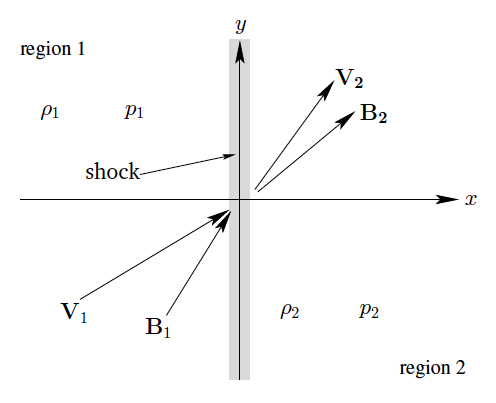
\includegraphics[scale=0.5, angle=0]{images/shock_pic}
\caption{Orientation of magnetic field and velocity field with respect to shock plane, in the rest frame of the shock. Shock normal in this case would be along the $-x$ direction i.e., into upstream region 1. \citep{fitz}}
\label{fig:shock_pic}
\end{center}
\end{figure}

The flow velocity $v$ and magnetic field $B$ are considered to be in the xy-plane. The appropriate conservation  equations are
\begin{subequations}
\begin{align}
&[\rho v_{x}]=0 \\
&[\rho v_{x}^2+p+\dfrac{B_{y}^2}{2\mu}]=0 \\
&[\rho v_{x}v_{y} - \dfrac{B_{x}B_{y}}{\mu}]=0 \\
&[\dfrac{1}{2}v^2 + \dfrac{\gamma p}{(\gamma-1) \rho}+\dfrac{ B_{y}(v_{x}B_{y} - v_{y}B_{x})}{\mu \rho v_{x}} ]=0 \\
&[B_{x}]=0 \\
&[v_{x}B_{y} - v_{y}B_{x}]=0 
\end{align}
\end{subequations}
These are the general MHD shock jump conditions where $v$ is the fluid velocity and $B$ is the magnetic field (with their corresponding components $\textquoteleft$x' or $\textquoteleft$y'), $\rho$ is the mass density, $p$ is the thermal pressure, and $\gamma$ is the ratio of specific heats (or the polytropic index). The meaning of the square brackets is $[F]\equiv F_{1}-F_{2}$, for any quantity F, and the $1$ or $2$ subscripts represent upstream or downstream values of each quantity F, respectively. These set of jump conditions differ only from the purely acoustic ones due the presence of the magnetic field. For example, taking (4a), (4b), and (4d) and setting $B_{x}=B_{y}=0$ we obtain the jump conditions for a neutral gas. Each conservation equation has a specific meaning; 
\begin{itemize}
\item (4a) is a mass conservation equation whereby the mass flux entering the shock must equal the mass flux leaving. It has units of kg\,m$^{-2}$\,s$^{-1}$.
\item (4b) indicates that if mass flux $\rho_{1} v_{x,1}$ enters the shock with momentum $(\rho_{1} v_{x,1})v_{x,1}$ it leaves the shock with momentum $(\rho_{1} v_{x,1})v_{x,2}$, the difference being equal to the the changing force per unit area across the shock. In this case both thermal and magnetic pressures contribute to change in momentum flux. (4c) implies the same process but relates the $x$ and $y$ components of the $v$ and $B$ vector fields. Both equations have units of momentum flux $\equiv$ (kg\,m$^{-2}$\,s$^{-1}$)(m\,s$^{-1}$) = (kg\,m\,s$^{-2}$m$^{-2}$) = N\,m$^{-2}\equiv$ pressure.
\item (4c) is an energy conservation term, accounting for the rate at which gas and magnetic pressure do work per unit area at the shock and equates this to the growth (or loss) in internal energy and kinetic energy across the shock. All components of magnetic field pressure are taken into in the last term on the left of the equation. All quantities are in units of J$\cdot$kg$^{-1}$.
\item (4d) simply states that the x component of the magnetic field i.e., the component of the field that is (anti-)parallel to the shock normal $\hat{n}$ is unaffected by the shock transition. 
\item (4f) relates the orientations of the upstream and downstream magnetic field to the flow speed tangential and perpendicular to the shock normal. Magnetic field orientation and hence the distribution of low speed amongst the velocity components largely depends on the whether the shock is slow-mode, intermediate, or fast mode. The equation has units of T$\cdot$m$\cdot$s$^{-1}$ = V$\cdot$m$^{-1}\equiv$ electric field.
\end{itemize}

4(a-f) are the general case of the jump conditions across an MHD shock, they are usually known as the MHD Rankine-Hugoniot (RH) equations. Their generality make the solution of the six unknowns from the six equations quite complicated. However the extreme cases of parallel and perpendicular shocks provide very useful and simplified expressions. It can be shown that parallel shocks i.e., $\hat{v}\parallel\hat{B}\parallel\hat{n}$ reduces to the jump conditions of a hydrodynamic shock in a neutral gas (here parallel and anti-parallel are used synonymously). The more interesting case when considering radiating shockwaves in the low solar corona is the perpendicular (or quasi-perpendicular) MHD shock, in this case the flow speed is parallel to the shock normal, and the magnetic field is perpendicular (or at a high angle) to it i.e., $\hat{v}\,\|\,\hat{n}$ and $\hat{B}\perp\hat{n}$. As will be shown it is this special case of quasi-perpendicular shocks that lead to efficient shock drift particle acceleration, a necessary precursor to the generation of radio emission at a coronal shockwave. 

In the case of fully $\perp$ shocks there is no need for the decomposition of the magnetic and velocity vector fields, meaning the $x$ and $y$ subscripts on 4(a) and 4(b) can be dropped. 4(c) is an obsolete jump condition, likewise for 4(e) since no $B_x$ field exists. We can also rid the $B_{x}B_{y}$ terms from the last quotient in the energy conservation 4(d) --replacing it simply with $B^{2}/2\mu\rho$. 4(f) reduces to a simpler form of $[Bv]=0$. Such a reduction in the generalized jump conditions allows us to express the upstream and downstream plasma properties in terms of the shock compression ratio $\chi=\dfrac{\rho_{2}}{\rho_{1}}$ as well as the upstream sonic Mach number $M_{1}=\dfrac{v_{1}}{c_{1}}$ \citep{priest2000} e.g.,
\begin{subequations}
\begin{align}
&\dfrac{v_{2}}{v_{1}}=\frac{1}{\chi} \\
&\dfrac{B_{2}}{B_{1}}=\chi \\
&\dfrac{p_{2}}{p{1}}=\gamma M_{1}^2\bigg(1-\frac{1}{\chi}\bigg) - \frac{1-\chi^2}{\beta_{1}}
\end{align}
\end{subequations}
where $\beta_{1}=2\mu p/B_{1}^2$ is the upstream plasma beta parameter. The exact value of the compression ratio may be obtained by using 4(b) to eliminate $p$ from the energy flux equation 4(d) and incorporating 4(a,c,e,f) (and a lot of algebra) a quadratic for $\chi$ may be obtained
\begin{equation}
2(2-\gamma)\chi^{2}+[2\beta_{1}+(\gamma-1)\beta_{1}M_{1}^2+2]\gamma\chi - \gamma(\gamma+1)\beta_{1}M_{1}^2=0
\end{equation}
%where $M_{1}$ is the upstream sonic Mach number, $\beta_{1}$ is the upstream beta parameter and, and $\gamma$ is the ploytropic index. 
Equation (6) has one positive real root such that 
\begin{equation}
1< \chi < \frac{\gamma+1}{\gamma-1}
\end{equation}

Using a ploytropic index of $\gamma=5/3$ (monatomic) means the shock compression can be no more than a factor of 4. Another extremely important fact arising from this is that magnetic compression can also be no greater than 4 i.e., from equation 4(b) $B_{2}/B_{1}=\chi$. $\chi<4$ has consequences for the shock drift acceleration mechanism and may also provide an upper limit to the level of band splitting in type II radio bursts (since this effect is thought to be related to the emission induced up/downstream of the shock). Although the maximum compression ration of 4 was derived from the roots of the quadratic for $\chi$ for the perpendicular shock, a similar analysis for the much more general oblique shock also leads to the same result. The density compression and tangential magnetic compression can be no more than a factor of $(\gamma+1)/(\gamma-1)$ for any MHD shock. 

%In either the perpendicular case or the general 2D oblique case a polynomial expression for the compression ratio (such as (6)) may be derived. The general oblique shock case requires extra terms in the polynomial such as $M_{A},\beta,\gamma,\theta_{Bn},\theta_{vn}$ ($\theta_{Bn}$ is the angle between shock normal and magnetic field, and $\theta_vn$ is the angle between shock normal and plasma flow). 
Polynomials such as (6) are extremely useful, and can lead to simple expressions for the Alfv\'{e}nic-Mach number in terms of $\chi$, in this case
\begin{equation}
M_{A}=\sqrt{\frac{\chi(\chi+5+5\beta)}{2(4-\chi)}} 
\end{equation}
for a perpendicular shock. If the shock speed and compression ratio are known, this equation provides a means of measuring the Alfv\'{e}n speed in the shock medium. 

This technique is exploited in the analysis of type II radio bursts. As the shock propagates into the corona it emits EM radiation at the local plasma frequency (1) (see section 4), and since the density drops as the shock travels into the heliosphere, so too does the frequency of emission. From frequency drift rate an estimate of shock speed is possible. If band splitting of the emission is present this is interpreted as emission from upstream and downstream of the shock, which provides a diagnostic of upstream/downstream densities via (1) and hence an estimate of $\chi$ \citep{vrsnak2002}. However, use of (8) in calculating Mach number and Alfv\'{e}n speed in the corona has some clear shortcomings such that it clearly ignores any dependency of the angle between magnetic field, velocity vector and shock normal i.e., (8) only applies to a purely perpendicular shock.

The general oblique shock case requires extra terms in the polynomial such as $\theta_{Bn}$ and $\theta_{vn}$ ($\theta_{Bn}$ is the angle between shock normal and magnetic field, and $\theta_{vn}$ is the angle between shock normal and plasma flow). For the oblique case the polynomial becomes
\begin{equation}
(A^2-\chi)^2\bigg[A^2 - \frac{2\chi S^2}{\chi+1-\gamma(\chi-1)}\bigg]\\
-\chi k^2A^2\bigg[\frac{2\chi - \gamma(\chi-1)}{\chi+1- \gamma(\chi-1)}A^2 -\chi\bigg]=0
\end{equation}
where $A=\frac{M_A\mathrm{cos}\theta_{vn}}{cos(\theta_{Bv}-\theta_{bn})}$,  $S=\frac{c_s}{v_A}$, $k=\mathrm{tan}(\theta_{vn}-\theta_{Bv})$ \footnote{$\theta_{Bv}$ is angle between magnetic field and velocity vector, it has a simple relationship with $\theta_{Bn}$} 
\citep{kabin2001}. Equation (6) is a quadratic of variable $\chi$, the more general equation (9) is a cubic equation for $\chi$, the roots of which give the compression for the oblique case. Since it is a function of $M_A$, $\theta_{vn}$, and $\theta_{bv}$, $\chi$ may have a range of values depending not only on Mach number but also shock orientation. Figure 2 illustrates the broad range in compressions of 0$<\chi<$3.5 across the shock depending on both flow and magnetic field orientation with respect to the shock normal, and in this case $M_A=2.5$. 
%\begin{figure}[h!]
%\includegraphics[scale=0.5, angle=270,trim =  3cm 0cm 4cm 0cm]{data/vary_thetaVn_thetaBn_mach2_5.pdf}
%\caption{Image and surface plot of compression ratio (from the solutions of (9)) as a function of $\theta_{vn}$ and $\theta_{Bn}$, with an Alfv\'{e}n Mach number of 2.5. The range of compressions is from 0 to 3.5 depending on the orientation of the magnetic field and velocity vectors with respect to the shock normal. Any discontinuities or sharp jumps are an indication of where the solutions to (9) are multi-valued.}
%\label{fig:vary_thetaVn_thetaBn_mach2_5}
%\end{figure}
This is a very general case, however, permitting any angle of orentation of $B$ and $v$. Since type II bursts are thought to be from shocks that are quasi perpendicular, this places restriction on the values for $\theta_{vn}$, and $\theta_{Bn}$, especially when the flow is considered to be head-on i.e. $\theta_{vn}=0^{\circ}$. Therefore in the quasi-perpendicular case their is a tighter constraint on the amount of compression across the shock. Further constraining the Mach number to a limited range of values puts quite a limiting range on the compression ratio, and hence a limiting range of band splitting of type II radio bursts since $f_{plasma}\approx9000\sqrt{n_e}$, hence
\begin{equation}
\delta_{bs} \equiv \frac{f_{upper}}{f_{lower}} \approx \sqrt{ \frac{ n_{e,d} }{ n_{e,u} } }=\sqrt{\chi}
\end{equation}
where $n_{e,d}$ and $n_{e,u}$ are downstream and upstream plasma number densities, and $\delta_{bs}$ is the ratio of upper to lower band frequencies, $f_{upper}$ and $f_{lower}$ respectively, in a split radio burst. Figure 3 shows the expected range in band splitting ($\delta_{bs}=\sqrt{\chi}$) for a type II given a range in Alfv\'{e}n Mach numbers $1<M_A< 4$, and quasi-perpendicular magnetic field orientations $45^{\circ}<\theta_{Bn}<90^{\circ}$. 
\begin{figure}[h!]
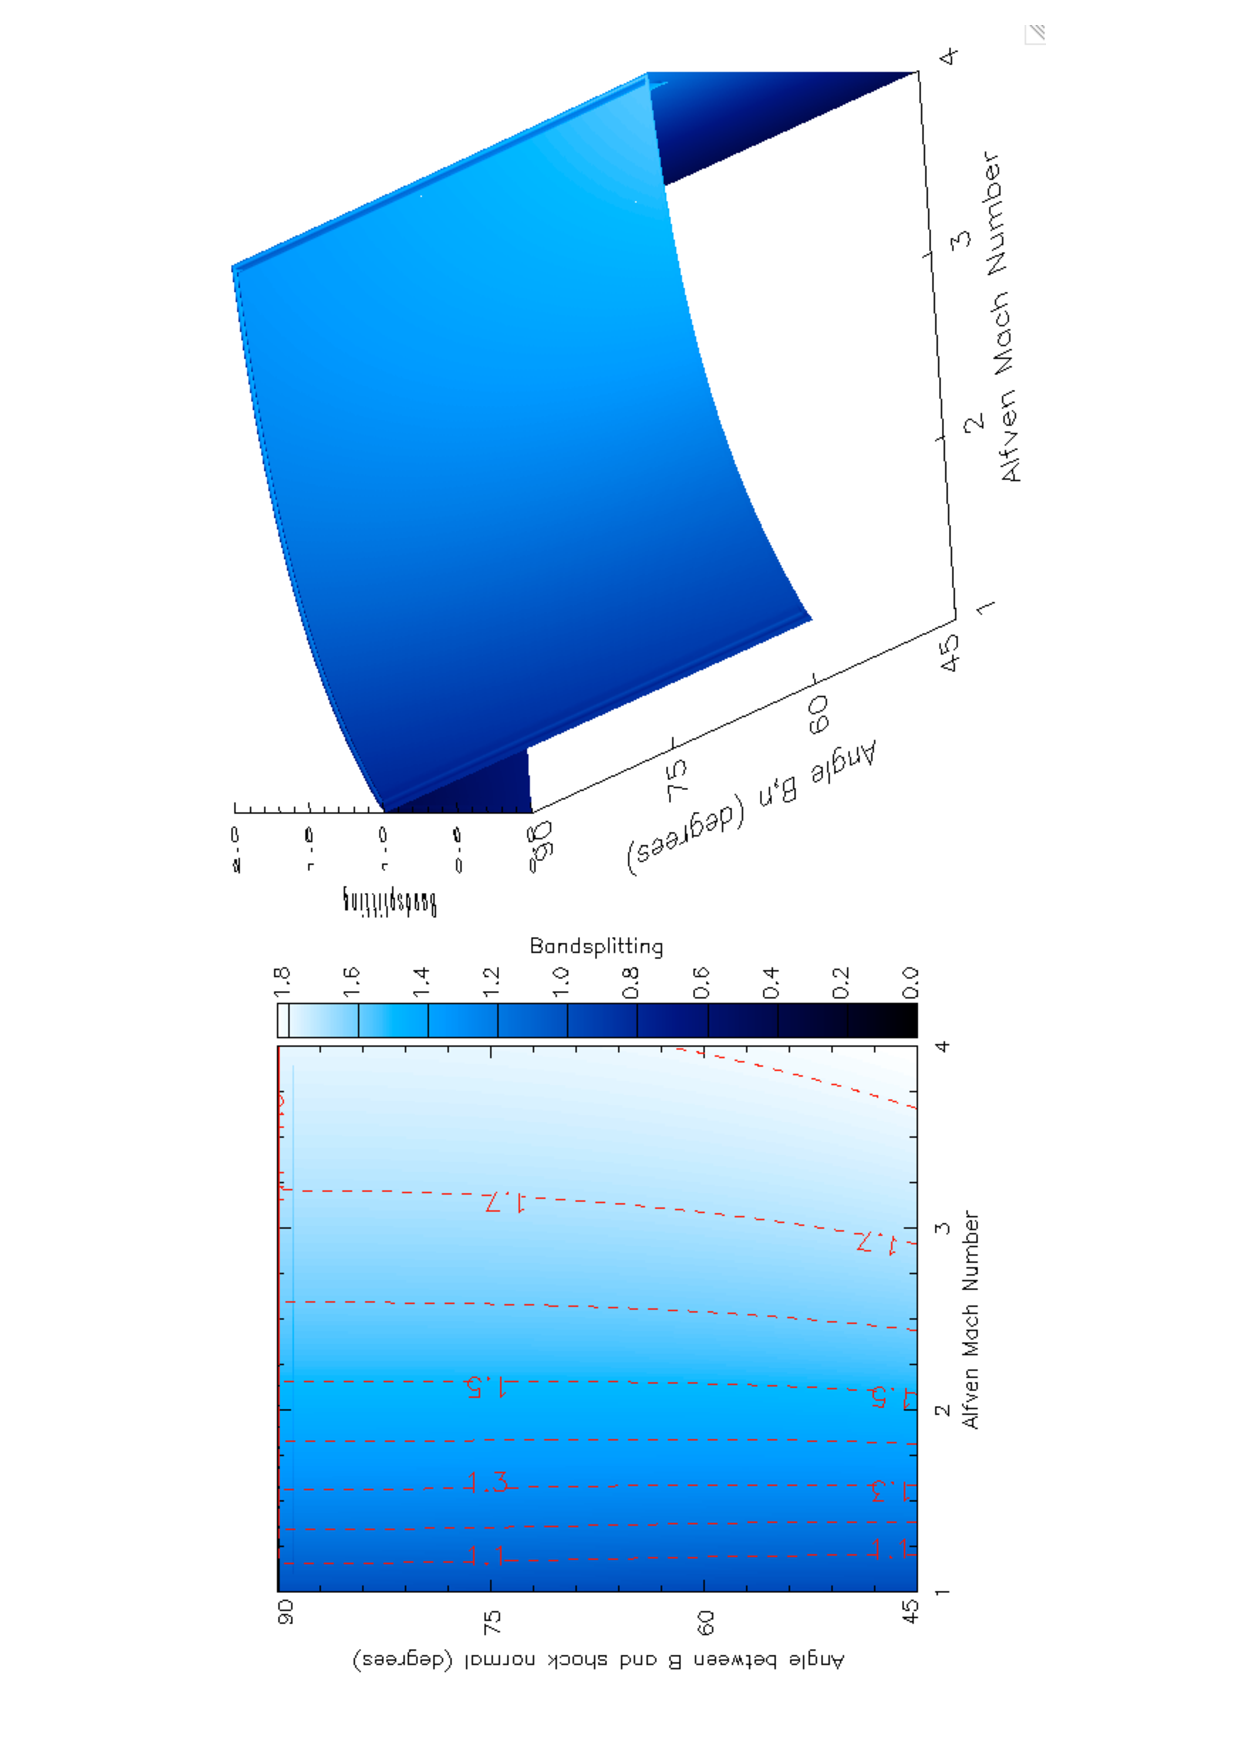
\includegraphics[scale=0.5, angle=270,trim =  3cm 0cm 4cm 0cm]{images/MHD_vary_mach&thetaBn.pdf}
\caption{Predicted band splitting ratio $\delta_{bs}$ as a function of Mach number and magnetic field orientation with respect to shock normal. Flow is anti-parallel to shock normal (head-on). Both image and surface are shown, left and right respectively. On the left, the red contours show specific values of of band-splitting. Note that for small mach numbers the level of band splitting is independent of magnetic field orientation. It is only at Mach numbers greater than $\sim$2.1 that the B-field orientation becomes important.}
\label{fig:MHD_vary_mach&thetaBn}
\end{figure}
This analysis shows that for a quasi-perpendicular shock the theoretically predicted range in type II band-spliting is $1<\delta_{bs}<1.8$. Such an upper limit to the level of band-splitting seems excessive and is probably due to a large upper limit to the Mach number being used to calculate the compression ratio. This is especially relevant in the low corona where Alfv\'{e}n speed can be quite large, making it difficult for a CME or blast wave to drive a shock at $M_A=4$. Also, given a typical band-splitting ratio of $\delta_{bs}=1.21\pm0.7$ at metric wavelengths \citep{vrsnak2004}, this would indicate typical Alfv\'{e}n-Mach number of $\sim\,1.5$ in the low corona. This seems reasonable, however Mach numbers of $\sim$3 are possible, and figure 3 would suggest a possible band-split ratio of $\delta_{bs}\sim1.7$ for such a Mach number. Such a level of band-splitting seems very unlikely, suggesting a quasi-perpendicular shock with a head on flow is a limiting case. More likely is a quasi-perpendicular shock with a flow orientation $\theta_{vn}\neq0$. For example if $\theta_{Bn}=90^{\circ}$ and $\theta_{vn}=45^{\circ}$ then band splitting can be $\delta_{bs}\sim\,1.5$ for $M_A$=3, which is under the upper limit of observed type II band-split ratios of $\sim\,1.58$. Allowing $\theta_{vn}\neq0$ can allow larger, more realistic Mach numbers to produce smaller and more realistic bandsplitting.


It is clear that the distribution in the level of band splitting in type II radio bursts depends not only on Mach number but the relative orientations of flow and magnetic field with respect to shock normal. A statistical analysis could possibly give an observationally predicted distribution in $\theta_{Bn}$ (provided $M_A$ is known) that would confirm the quasi-perpendicularlity of type II-generating shocks.

%\subsection{Bow Shocks}\label{sec:15}



\section{Coronal Mass Ejections}\label{sec:2}

\subsection{Catastrophe Model}\label{sec:20}

\subsection{Magnetic Breakout Model}\label{sec:21}

The magnetic breakout model was first proposed by \citep{antiochos1999} and involves a quadrupolar (or more complex) magnetic flux system. A core magnetic field is flanked by two side-lobe fields, which collectively lie underneath an over-arching field that stabilizes the whole system. The overarching field and core field are almost anti-parallel, creating a magnetic null point between the two Figure~\ref{fig:breakout_model}. Non potentiality is injected into the core by twisting/shearing of the foot points or by flux emergence. This non-potentiality causes the core field to grow and encounter the overarching field, distorting the null point into a current sheet and eventually allowing reconnection to occur. The reconnection removes field lines from the overarching field and adds it to the side-lobe systems, allowing further growth of the core field. The growth of the core field in turn drives further breakout reconnection resulting in a positive feedback required for explosive expulsion of the core. Finally, as the core is accelerated a current sheet forms in its wake, eventually leading to a separation of the core flux from the solar surface that forms a plasmoid structure typical of a three part CME \citep{lynch2004}; an important aspect of this is that flux rope formation happens as a consequence of eruption i.e., it is not pre-existing. The magnetic breakout model was used to circumvent the Aly-Sturrock limit \citep{aly1991, sturrock1991} i.e., it allowed a flux system to erupt, without having to open the constraining field lines to infinity.
\begin{figure}[!b]
\begin{center}
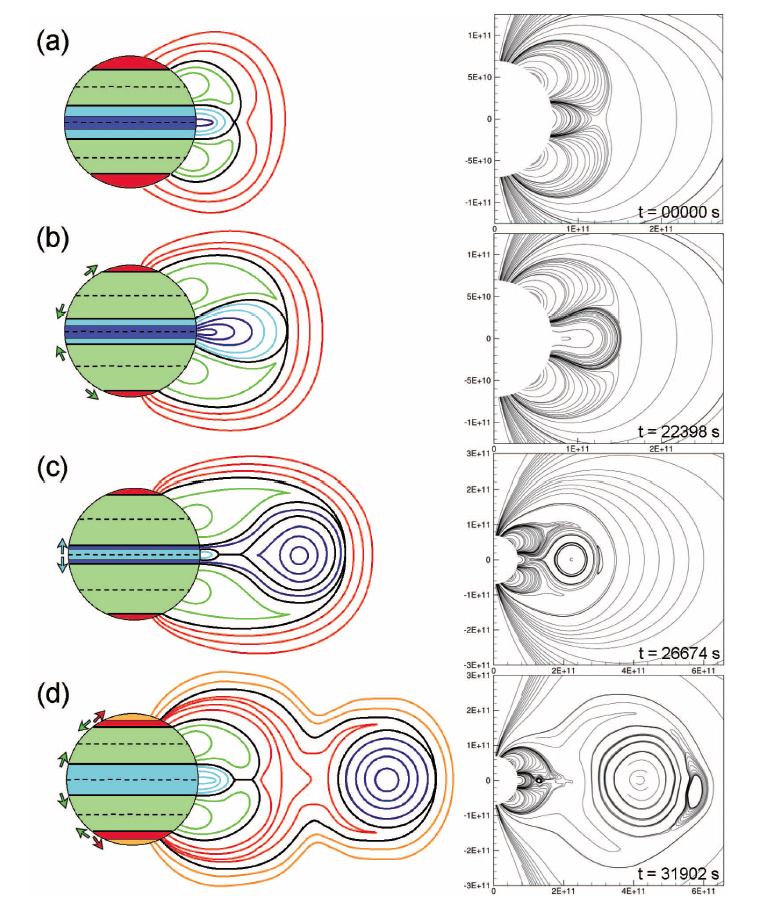
\includegraphics[scale=0.55]{images/lynch_breakout}
\caption{The breakout model, consisting of a quadrupolar flux system in which the central flux (blue) is flanked by to side lobe flux systems (green), with the entire system kept in stability by the tension of the overlying red field. Shearing and/or twisting on the underlying flux causes it to grow slowly. Eventually a current sheet forms at the magnetic null above the central flux, causing reconnection. This reconnection transfers overlying field to the side-lobes, effectively creating a conduit for the central flux to escape as a CME \citep{lynch2008}.}
\label{fig:breakout_model}
\end{center}
\end{figure}
\clearpage
Kinematically, the CME/central field system should experience a slow rise (1\,km\,s$^{-1}$) for several hours due to shearing/twisting of the foot points. Once breakout reconnection has begun the CME experiences a much larger acceleration (100\,km\,s$^{-1}$). The reconnection in the current sheet in the wake of the CME is the source of energetic particles that ultimately lead to flaring (ribbons and soft x-ray loops). Therefore magnetic breakout predicts that the flaring process and SXR peak should only begin after CME acceleration (after breakout reconnection) has begun \citep{lynch2004}. However, the precedence in breakout reconnection over flaring reconnection may not always be case, with the latter sometimes driving the former \citep{macneice2004}. 

There has been observational tests of the magnetic-breakout model, showing it to be a viable explanation of some flaring and CME events, the most notable of which is the Bastille Day event \citep{aulan2000}. The observational signatures of the model include the presence of a null point in the corona above a complex multipolar flux system (inferred from potential field source surface extrapolations), a radio source imaged to be above the erupting structure (implying a reconnection site), and radio bursts beginning at frequencies indicative of high altitude (again indicating energy release above the erupting structure, prior to eruption) \citep{mano2003}. However, in some instances magnetic breakout is implied by observations of the above, but the kinematics are inconsistent with model predictions. For example the model predicts a long slow rise of the central flux system as the underlying field is increasingly sheared, after which there is a rapid acceleration once breakout reconnection is initiated. However, in the study of \citet{bong2006} the breakout reconnection occurred at the end of the CME acceleration phase, prompting a two-phase acceleration scenario.


\subsection{Toroidal Instability}\label{sec:22}

The toroidal instability model incorporates a pre-existing flux rope structure that is built from a torus of magnetic flux, some of which is buried beneath the photosphere \citep{chen1989}. The flux system is can be broken down into a combination of toroidal magnetic, toroidal current and a poloidal magnetic field and current Figure~\ref{fig:chen_model}. This flux rope system is embedded in a surrounding coronal magnetic field $B_{corona}$. The stability of the system depends on the nature of the $J \times B$ force due to the interaction toroidal and poloidal components of both the field and current. The interaction of $J$ and $B$ internal to the flux rope is usually termed the Lorentz self-force or the \textquoteleft hoop' force. An instability may be induced via twisting of the fluxrope footpoints to increases the amount of poloidal flux (effectively increasing the helicity of the system). The instability arrises when the outward hoop force decreses more slowly within the ring radius than the opposing Lorentz force due to an external magnetic field. Once the instability is induced, the fluxrope begins a bulk motion as well as a growth in its semi-minor axis. Hence the motion of the system can be analysed by looking at the central axis or the minor axes (leading and trailing edges. The three axes display slightly different kinematics e.g., the leading edge has a faster velocity than the trailing edge (due to fluxrope expansion). this has proved a useful test of the model when comparing the observations of erupting fluxrope structures as seen in white-light coronagraphs. \citet{krall2001} looked at the leading a trailing edges of erupting flux ropes, as well as the rope aspect ratio, an compared the observations to model expectations. Good agreement is found between the model kinematics and aspect ratio and the observed events.
\begin{figure}[!t]
\begin{center}
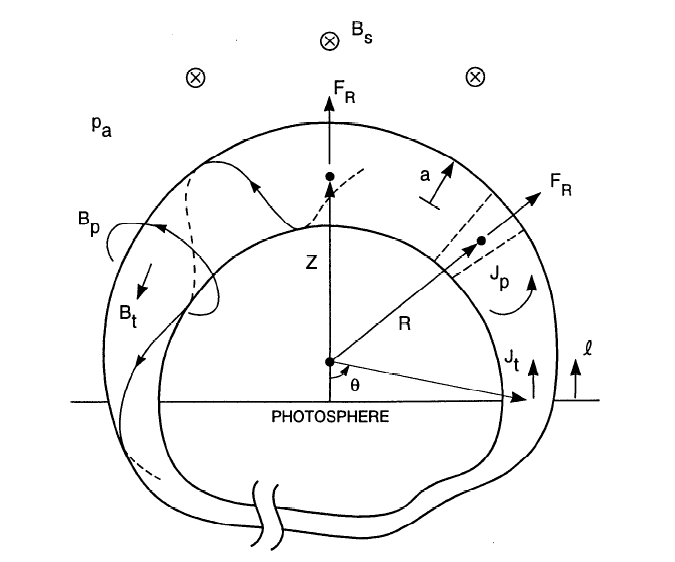
\includegraphics[scale=0.5]{images/chen_model}
\caption{The flux rope model of \citet{chen1989}, used to to study the toroidal instability of a twisted flux system in the corona.}
\label{fig:chen_model}
\end{center}
\end{figure}
The equation of motion of the entire system is given by
\begin{equation}
M\frac{d^2Z}{dt^2} = \frac{I_t}{c^2R}\times\bigg[ \mathrm{ln}\bigg(\frac{8R}{a}\bigg) -1+ \frac{\xi_i}{2} + \frac{\beta_p}{2} -\frac{B^2_t}{B^2_{pa}}  -\frac{2RB_{\perp c}}{aB_{pa}} \bigg] - F_g - F_{drag}
\end{equation}
where $I_t$ is the toroidal current, $R$ is the flux rope major radius, $a$ is the rope minor radius, $\xi_i$ is internal inductance of the flux system, $B_t$ is the toroidal field, $B_{pa}$ is the poloidal field at $a$, $B_{\perp c}$ is the perpendicular component of the ambient coronal field, $F_g$ is the force due to gravity, $F_{drag}$ is the drag force, $M$ is the mass per unit length of the rope, and $Z$ is the rope axis height above the photosphere. The equation of motion shows that an increase in the toroidal current (or poloidal flux) contributes positively to the acceleration. The terms in the square brackets are each unitless and take into account the rope geometry, self-inductance and interplay between poloidal and toroidal flux. The first three terms in the square brackets are what give rise to the hoop-force. If the rope is mass loaded with a prominence, this can contribute to the rope's stability via the gravity term. The drag term only becomes an important contributor to rope dynamics later in the propagation, when the solar wind speed begins to increase i.e., at around 10$R_{\odot}$ reference Sheeley. The eruption is driven by flux-injection, which typically lasts for 4-8 hours, during which time the unstable system loses its equilibrium and begins to rise \citet{krall2001}.

It is significant the fluxrope is already established in the corona before eruption begins i.e., the rope formation is not addressed in the model and it is not a consequence of eruption. Hence magnetic reconnection is not a necessary aspect of the model and the eruption may proceed without employing resistive MHD. The model has been tested against observations and found to provide consistent result with the acceleration and jerk profiles of destabilized filaments during eruption \citep{schrijver2008}


\subsection{Drag Models}\label{sec:23}


\section{Coronal Shocks and Plasma Emission}\label{sec:3}

\subsection{Shock Particle Acceleration}\label{sec:30}

\subsection{Wave-Particle Interaction}\label{sec:31}

Distributions of particles in a plasma can give rise to resonances in various wave modes. In general we may relate a particle distribution function in velocity space $f(v_{\|})$ with a distribution function of wave modes in wave-number or $\textquoteleft\mathbf{k}$-space' $N(\mathbf{k})$
\begin{equation}
\frac{\partial N(\mathbf{k})}{\partial t}+v_{g}(\mathbf{k})\frac{\partial N(\mathbf{k})}{\partial r} = \Gamma(\mathbf{k},f(v_{\|}))N(\mathbf{k})
-\Gamma_{coll}(\mathbf{k}) N(\mathbf{k})
\end{equation}
where the lefthand side takes the form of a Lagrangian derivative with group speed $v_g$, $\Gamma$ represents a wave growth term given the distribution function $f(v_{\|})$, and $\Gamma_{coll}$ is a term taking into account collisional damping of the wave \citep{aschbook}.

In order to see how the distribution function effects wave growth we start with an equilibrium distribution $f_0$ and impose a perturbation $f_1(r,v,t)$, so that the total distribution function is $f(r,v,t) = f_0 +f_1(r,v,t)$. Note that the only contribution to the electric field $\mathbf{E}$ is from perturbed quantities and a relationship between $f_1$ and electric field $\mathbf{E}$ may be obtained using Poisson's equation, And by assuming solutions for the perturbation quantities only of type $e^{j(\omega - \mathbf{k\cdot x})}$ we have
\begin{equation}
-i \mathbf{k}\cdot \mathbf{E}=\frac{q_e}{\epsilon_0}\int_v f_1d^3v
\end{equation}
Now, using $f(r,v,t)$ in the Vlasov equation and linearizing we obtain
\begin{equation}
f_1=\frac{q_e}{m_e}\frac{j}{\omega-\mathbf{k\cdot v}}\mathbf{E}\cdot\nabla_vf_0
\end{equation}
Integrating both sides of (20) over all velocity space and using (19) the general form of the dispersion relation of the oscillations $(\omega,\mathbf{k})$ in perturbations $f_1$ and $E$ is derived
\begin{equation}
1+\frac{q_e}{\epsilon_0m_e}\frac{1}{k}\mathbf{k}\cdot\int_v\frac{\nabla_v f_0}{\omega-\mathbf{k\cdot v}}d^3v=0
\end{equation}
For a given background distribution $f_0$ this is function relates $\omega$ and $\mathbf{k}$ \citep{gol2011}. For a cold plasma such that $f_0$ is simply a delta function this expression leads to the familiar dispersion relation
\begin{equation}
\omega_{p}=\bigg(\frac{e^2n_e}{\epsilon m_e}\bigg)^\frac{1}{2}
\end{equation}
which is the electron plasma oscillation. For warm plasma $f_0$ e.g., for a maxwell velocity distribution but imposing an upper limit on the integral of $v_{max} < \omega/k$ (this is to avoid singularities in the integrand) the dispersion relation then yields $\omega^2=\omega_{p}^2+c_s^2k^2$ which is the dispersion relation for the Langmuir wave. This is very much the same as the plasma oscillation but with a very small group velocity imposed on the oscillation.

It can be shown that (21) is also the effective dielectric permittivity of the plasma as a function of $(\omega,\mathbf{k})$. Therefore (21) expressed more simply is
\begin{equation}
\epsilon_{eff}(\omega,\mathbf{k})=0
\end{equation}
The general solution requires integration of (21) over all velocities. This is not a trivial integral since at $v = \omega/k$ the integrand become infinite. In order to perform the integration the integrand is evaluated normally everywhere that is not in the vicinity of the singularity, these evaluations lead to a real part of $\epsilon_{eff}$, namely $\epsilon_r$. Close to the singularity ($v \sim \omega/k$) the integrand is evaluated at values approaching but never exactly on $v = \omega/k$, these evaluations lead to an imaginary part of $\epsilon_{eff}$, namely $j\epsilon_i(\omega,\mathbf{k})$ \citep{melrose1989}. Such an integration needs to be done on a complex plane and the resultant solutions for $\epsilon_{eff}(\omega,\mathbf{k})$ are generally complex
\begin{equation}
\epsilon_{eff}(\omega,\mathbf{k})=\epsilon_r(\omega,\mathbf{k})+j\epsilon_i(\omega,\mathbf{k})
\end{equation}
The solutions $\epsilon_r(\omega,\mathbf{k})$ are real $\omega_r$, and give the dispersion relations as normal. The $\epsilon_i(\omega,\mathbf{k})$ solutions are complex dispersion relations, such that the general solutions of (21) or (23) will be
\begin{equation}
\omega = \omega_r + j\omega_i
\end{equation}
The complex $j\omega_i$ means that the time dependency of the periodic solutions to the perturbations $f_1$ and $\mathbf{E}$ will be $e^{j\omega t}=e^{(j[\omega_r + j\omega_i])}=e^{j\omega_rt}e^{-\omega_it}$. This solution is a damped wave with damping factor $\omega_i$, meaning the solutions to (21) in the region $v \sim \omega/k$ provide a wave decay term. However, since the damping term is dependent on the negative of the velocity space gradient $\omega_i \sim -\nabla_v f_0$\footnote{Proof of this statement requires integration analysis along specific contours in the complex plane and is usually done with the use of a Laplace transform (and is very long winded!)} \citep{melrose1989}, a positive gradient in the velocity distribution function provides negative damping i.e., wave growth, meaning $\omega_i \equiv \Gamma$ in this instance. Hence the positive gradient provided by the shock drift accelerated beam of electrons results in the growth of waves.

In effect, shock drift acceleration promotes a group of electrons to a velocity range that closely matches the phase speed of some type of waves in a medium $v \sim \omega/k$. In such a speed range the integrand of (21) approaches the point at which there is a singularity in the solution. Such a point necessitates a complex solution to the integral, thus providing an imaginary part to the dispersion relation that gives an $e^{-\omega_it}$ term. If the promotion of electrons to a range $v \sim \omega/k$ is combined with a positive gradient of the distribution function in this velocity range, it results in $\omega_i < 0$ and $e^{-\omega_it}>0$, leading to wave growth. This is why $v - \omega/k=0$ is known as the resonance condition. Since electron beams in the corona match the phase speed of Langmuir waves in the corona, the beam results in the generation of Langmuir waves. So for shock drift accelerated electron beams to excite Langmuir waves $v_{beam}=\sqrt{\frac{\omega_p^2}{k^2} +c_s^2}$. A term for gyro-resonance needs to be added to this if the plasma is magnetized.

Once the Langmuir waves are generated a process known as quasi-linear relaxation occurs whereby part of the energy in the beam electrons is acquired by the Langmuir waves. In the simplest case of a delta function beam the system evolves to state whereby 2/3 of the initial beam kinetic energy $\frac{1}{2} m_e n_b v_b^2$ is fed into the waves, while the remaining 1/3 is retained by the electrons. This results in the distribution of the electrons migrating to lower energy (lower v) and a flattening of the beam in phase space. Once the beam is flattened into a plateau the phase space gradient vanishes and their is no longer a growth of Langmuir waves. This process is known as quasi-linear relaxation and represents a return to stability. %Schmidt 2012


\begin{figure}[!t]
\begin{center}
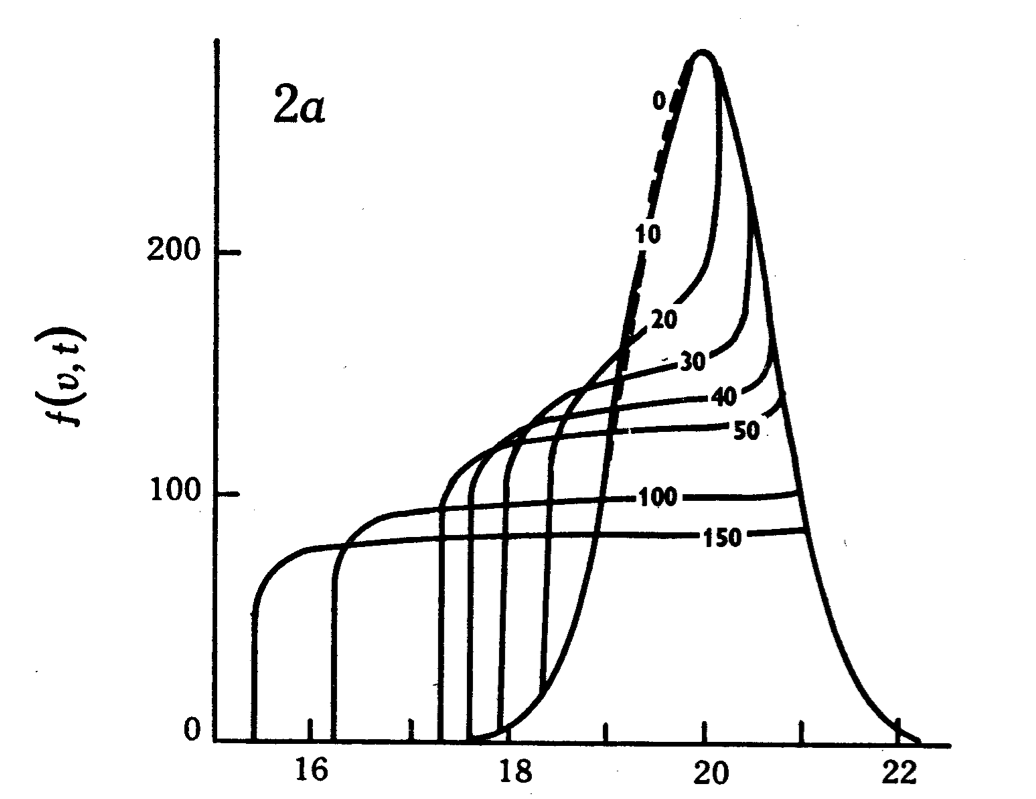
\includegraphics[scale=0.35, trim = 4cm 0cm 0cm 0cm]{images/Grognard1975}
\end{center}
\end{figure}


\subsection{Three-Wave Interaction and Plasma Emission}\label{sec:32}

Once the Langmuir waves are produced from the bump-on-tail instability a number of wave interaction processes occur in order to bring about plasma emission. This involves the interaction of various wave modes in the plasma described by a mathematical formalism called the three-wave interaction. In this process three wave modes in a plasma M, P, and Q are described by their distribution functions in a wave-number space ($k$-space). the distribution functions are given by $N_M(k_M)$, $N_P(k_P)$, $N_Q(k_Q)$, where the $N$ describe the occupation number of wave quanta between $k$ and $k+dk$ in the wave-number space. Waves in P and Q mode may interact to such that wave quanta are removed from the P and Q k-space and added to the M k-space. This is essentially an emission of an energy packet from the P and Q -space to the M k-space. The rate of change of occupation numbers in the three k-spaces are given by
\begin{equation}
\frac{dN_M(\mathbf{k}_M)}{dt} = -\int \frac{d^3\mathbf{k}_P}{(2\pi)^3}\int \frac{d^3\mathbf{k}_Q}{(2\pi)^3}g(\mathbf{k}_M, \mathbf{k}_P, \mathbf{k}_Q)
\end{equation}
\begin{equation}
\frac{dN_P(\mathbf{k}_P)}{dt} = -\int \frac{d^3\mathbf{k}_M}{(2\pi)^3}\int \frac{d^3\mathbf{k}_Q}{(2\pi)^3}g(\mathbf{k}_M, \mathbf{k}_P, \mathbf{k}_Q)
\end{equation}
\begin{equation}
\frac{dN_Q(\mathbf{k}_Q)}{dt} = -\int \frac{d^3\mathbf{k}_M}{(2\pi)^3}\int \frac{d^3\mathbf{k}_P}{(2\pi)^3}g(\mathbf{k}_M, \mathbf{k}_P, \mathbf{k}_Q)
\end{equation}
where $g(\bf{k}_M, \bf{k}_P, \bf{k}_Q)$ is incorporates a transition probability for wave quanta into and out of energy states in the various k-spaces \citep{robinson1994}. The transition probability is given by
\begin{multline}
g(\mathbf{k}_M, \mathbf{k}_P, \mathbf{k}_Q) = u_{MPQ}(\mathbf{k}_M, \mathbf{k}_P, \mathbf{k}_Q)   [N_M(\mathbf{k_M}) N_P(\mathbf{k_P})  - \\ 
N_P(\mathbf{k_P}) N_Q(\mathbf{k_Q})   +N_Q(\mathbf{k_Q}) N_M(\mathbf{k_M})  ]
\end{multline}
where $u_{MPQ}(\bf{k}_M, \bf{k}_P, \bf{k}_Q) $ is the transition probability from states in P and Q  to M, for example \citep{melrose1986}. $u_{MPQ}$ is analogous to transition probabilities given by the Einstein coefficients for transferring energy packets from and atomic state to a photon state (photon emission) i.e., whereas the Einstein coefficients are used in atom-wave (atom-photon) energy exchanges, $u_{MPQ}$ describes wave-wave energy exchanges. The transition probability is given by
\begin{equation}
u_{MPQ}(\mathbf{k}_M, \mathbf{k}_P, \mathbf{k}_Q)  \propto \delta(\omega_M - \omega_P - \omega_Q ) \delta^3(\mathbf{k}_M - \mathbf{k}_P - \mathbf{k}_Q )
\end{equation}
where the $\omega$ are the frequency of the corresponding wave and and $\delta$ are delta functions. Given the presence of delta functions in the transition probability expression, we can see that an exchange of energy quanta amongst the wave modes can only occur when 
\begin{eqnarray}
\omega_M & = & \omega_P + \omega_Q \\
\mathbf{k}_M & = & \mathbf{k}_P + \mathbf{k}_Q
\end{eqnarray}

Hence for an a conversion wave modes in a plasma such as $M \rightarrow P + Q$ (a decay of mode M into P and Q), or it's reverse process $P + Q \rightarrow M $ (a coupling of P and Q to produce M) is described by equations (2.1) to (2.7). 

The production of plasma emission after a bump-on-tail instability has occurred requires a three wave interaction amongst a Langmuir wave $L$, ion acoustic wave $S$, and electromagnetic wave $T$. Fundamental emission during a radio burst occurs via a decay of Langmuir waves into an electromagnetic and ion sound wave
\begin{equation}
L \rightarrow T + S
\end{equation}
while second harmonic first requires the decay $L\rightarrow L^{'} + S$, where $L^{'}$ is a product Langmuir wave propagating in the opposite direction to the first. This is followed by a coalescence of the original and product Langmuir waves
\begin{equation}
L + L^{'}\rightarrow T'
\end{equation}


\begin{itemize}
\item The dispersion relations
\item Source emissivities
\end{itemize}


